\documentclass{article}

\usepackage{graphicx}
\usepackage{tikz}
\usepackage{tikzsymbols}
\usetikzlibrary{calc,patterns,shapes.geometric}
\pagestyle{empty}
\usepackage[margin=0pt]{geometry}
\geometry{papersize={14in,12in}}

\def\centerarc[#1](#2)(#3:#4:#5){\draw[#1] ($(#2)+({#5*cos(#3)},{#5*sin(#3)})$) arc (#3:#4:#5);}

\begin{document}
	\begin{figure}
		\centering
		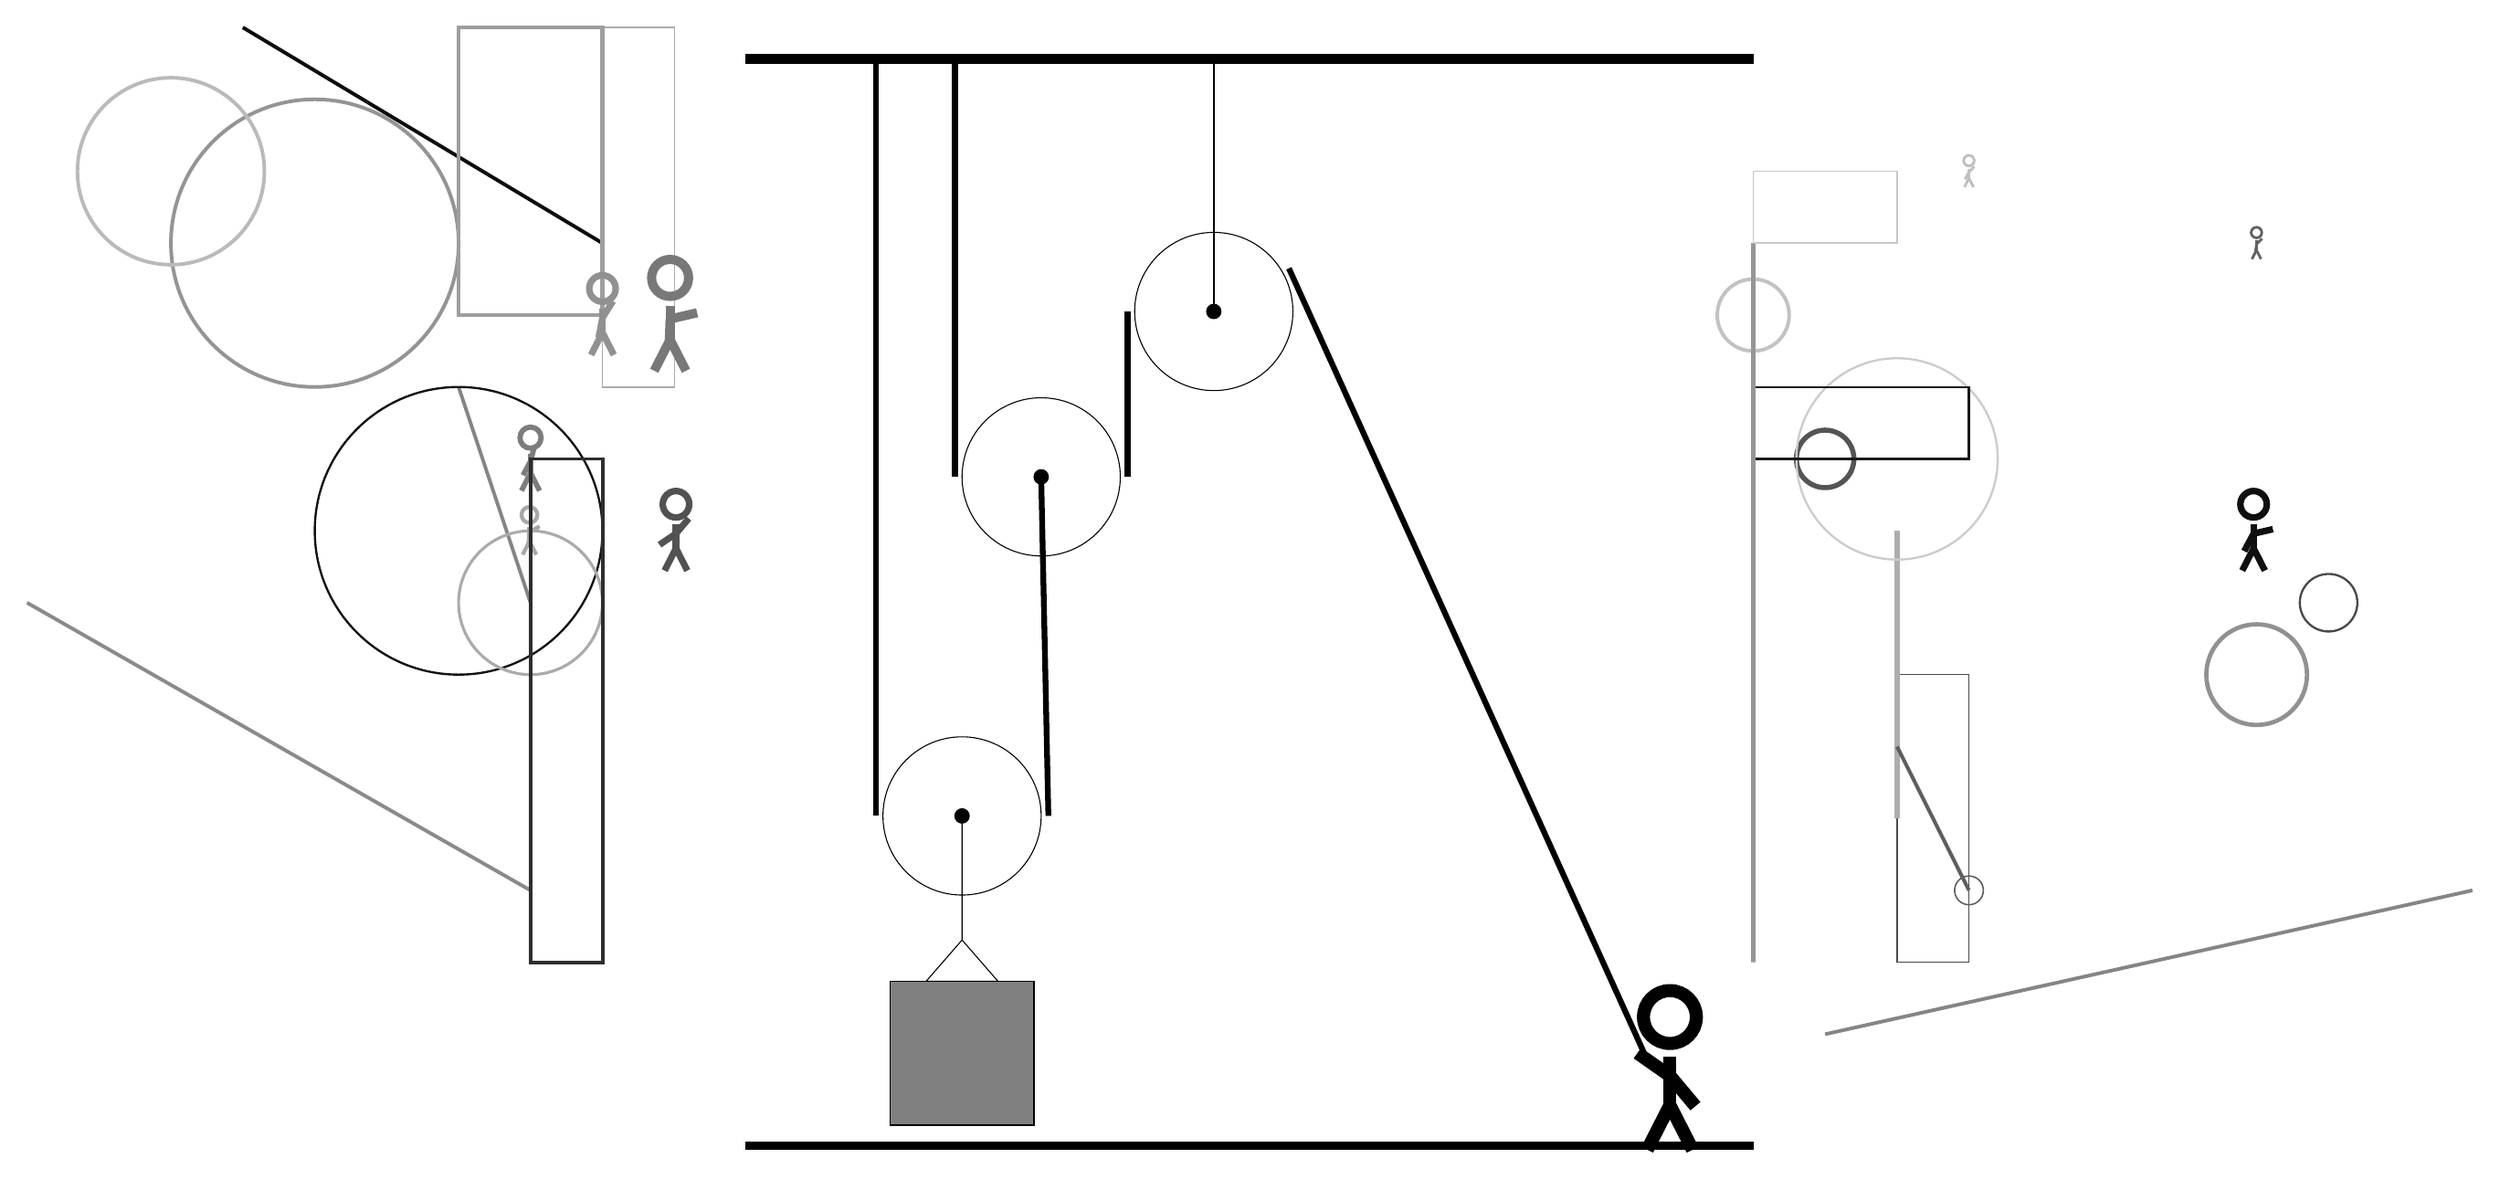
\begin{tikzpicture}
			%%%%% START %%%%%
			
			\draw[fill=black] (-2, 11.5) rectangle (12, 11.625);
			
			\draw (1, 1.035) circle (1.1);
			\draw[fill=black] (1, 1.035) circle (0.1);
			
			\draw (2.1, 5.75) circle (1.1);
			\draw[fill=black] (2.1, 5.75) circle (0.1);
			
			\draw (4.5, 8.05) circle (1.1);
			\draw[fill=black] (4.5, 8.05) circle (0.1);
			\draw[thick] (4.5, 8.05) -- (4.5, 11.5);
			
			\draw [line width=0.7mm, color=black!67](13, 6) circle (0.4);
			
			\draw [line width=0.5mm, color=black!42](-8, 9) circle (2.0);
			\draw[line width=0.2mm, color=black!71] (14, -1) rectangle (15, 3);
			\node[line width=0.2mm, color=black!34] at (-5, 5) {\Strichmaxerl[3][85][32]};
			
			\draw[line width=0.7mm, color=black!32] (14, 1) rectangle (14, 5);
			\draw[line width=0.2mm, color=black!33] (-3, 7) rectangle (-4, 12);
			
			\draw[line width=0.5mm, color=black!95](-4, 9) -- (-9, 12);
			
			\draw [line width=0.2mm, color=black!64](15, 0) circle (0.2);
			\draw[line width=0.5mm, color=black!48](-6, 7) -- (-5, 4);
			\draw [line width=0.3mm, color=black!93](-6, 5) circle (2.0);
			\draw[line width=0.6mm, color=black!46] (-2, 4) rectangle (-2, 4);
			\draw[line width=0.5mm, color=black!63](14, 2) -- (15, 0);
			\node[line width=0.6mm, color=black!62] at (19, 9) {\Strichmaxerl[2][82][45]};
			
			\node[line width=0.6mm, color=black!94] at (19, 5) {\Strichmaxerl[5][62][13]};
			\draw [line width=0.5mm, color=black!27](-10, 10) circle (1.3);
			\draw[line width=0.6mm, color=black!38] (-4, 12) rectangle (-6, 8);
			\draw [line width=0.6mm, color=black!43](19, 3) circle (0.7);
			\draw [line width=0.5mm, color=black!24](12, 8) circle (0.5);
			\draw [line width=0.3mm, color=black!20](14, 6) circle (1.4);
			
			\draw[line width=0.3mm, color=black!90] (12, 6) rectangle (15, 7);
			\draw[line width=0.6mm, color=black!41] (12, -1) rectangle (12, 9);
			
			\node[line width=0.6mm, color=black!53] at (-3, 8) {\Strichmaxerl[7][88][13]};
			\draw[line width=0.5mm, color=black!48](13, -2) -- (22, 0);
			\draw[line width=0.5mm, color=black!46](-5, 0) -- (-12, 4);
			\node[line width=0.4mm, color=black!25] at (15, 10) {\Strichmaxerl[2][60][48]};
			
			\node[line width=0.7mm, color=black!51] at (-5, 6) {\Strichmaxerl[4][62][75]};
			\draw [line width=0.4mm, color=black!33](-5, 4) circle (1.0);
			\draw[line width=0.2mm, color=black!21] (14, 9) rectangle (12, 10);
			\draw[line width=0.5mm, color=black!82] (-4, -1) rectangle (-5, 6);
			\node[line width=0.5mm, color=black!43] at (-4, 8) {\Strichmaxerl[5][79][58]};
			\node[line width=0.5mm, color=black!68] at (-3, 5) {\Strichmaxerl[5][34][50]};
			
			\draw [line width=0.3mm, color=black!71](20, 4) circle (0.4);
			
			\draw (1, 1.035) -- (1, -0.69) -- (0.5, -1.265) -- (1.5, -1.265) -- (1, -0.69);
			\draw[fill=black!50] (0, -1.265) rectangle (2, -3.265);
			
			\draw[line width=0.8mm] (-0.2, 11.5) -- (-0.2, 1.035);
			\centerarc[line width=0.8mm](1, 1.035)(180:360:1.2000000000000002);
			\draw[line width=0.8mm](2.2, 1.035) -- (2.1, 5.75);
			\draw[line width=0.8mm] (0.9, 11.5) -- (0.9, 5.75);
			\centerarc[line width=0.8mm](2.1, 5.75)(180:360:1.2000000000000002);
			\draw[line width=0.8mm](3.3, 5.75) -- (3.3, 8.05);
			\centerarc[line width=0.8mm](4.5, 8.05)(30:180:1.2000000000000002);
			\draw[line width=0.8mm] (5.544, 8.65) -- (10.5, -2.3);
			
			\node at (10.8, -2.5) {\Strichmaxerl[10][-35][-50]};
			
			\draw[fill=black] (-2, -3.5) rectangle (12, -3.6);
			
			%%%%% END %%%%%
		\end{tikzpicture}
	\end{figure}	
\end{document}